% fig_tdcs_delta_I.tex
% Bar chart: TDCS ΔI_rms vs k_ibr — 3PH internal fault study
% Two groups: 87L catches (green) and TDCS-only catches (yellow)
% Horizontal: Δ_thr = 0.04 pu, 87L threshold = 0.12/sqrt(2) ≈ 0.0849 pu (RMS equiv.)
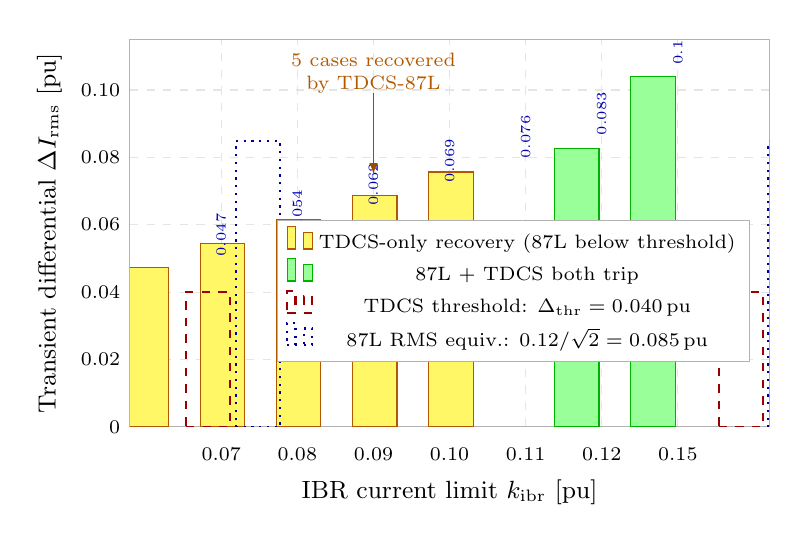
\begin{tikzpicture}
\begin{axis}[
  name        = tdcsax,
  ybar,
  bar width   = 16pt,
  width       = 0.80\textwidth,
  height      = 6.5cm,
  ylabel      = {Transient differential $\Delta I_{\rm rms}$ [pu]},
  ylabel style= {font=\small},
  xlabel      = {IBR current limit $k_{\rm ibr}$ [pu]},
  xlabel style= {font=\small},
  ymin=0, ymax=0.115,
  ytick       = {0, 0.02, 0.04, 0.06, 0.08, 0.10},
  yticklabels = {0, 0.02, 0.04, 0.06, 0.08, 0.10},
  yticklabel style={font=\scriptsize},
  xtick       = {1,2,3,4,5,6,7},
  xticklabels = {0.07, 0.08, 0.09, 0.10, 0.11, 0.12, 0.15},
  xticklabel style={font=\scriptsize},
  enlarge x limits=0.10,
  legend style={at={(0.97,0.35)}, anchor=east,
                font=\scriptsize, draw=gray!60},
  grid         = major,
  grid style   = {gray!20, dashed},
  tick style   = {draw=none},
  axis line style={gray!60},
]

% TDCS-only recoveries (k_ibr = 0.07–0.11): 87L misses but TDCS trips
\addplot[fill=yellow!60, draw=orange!70!black]
  coordinates {
    (1, 0.04738)
    (2, 0.05445)
    (3, 0.06152)
    (4, 0.06859)
    (5, 0.07566)
  };
\addlegendentry{TDCS-only recovery (87L below threshold)}

% 87L catches (k_ibr = 0.12, 0.15): both 87L and TDCS trip
\addplot[fill=green!40, draw=green!70!black]
  coordinates {
    (6, 0.08273)
    (7, 0.10394)
  };
\addlegendentry{87L + TDCS both trip}

% TDCS threshold = 0.04 pu
\addplot[red!60!black, thick, dashed, mark=none, domain=0.5:7.5, samples=2]
  ({x}, {0.040});
\addlegendentry{TDCS threshold: $\Delta_{\rm thr}=0.040$\,pu}

% 87L threshold (RMS equivalent of 0.12 pu peak)
\addplot[blue!60!black, thick, dotted, mark=none, domain=0.5:7.5, samples=2]
  ({x}, {0.08485});
\addlegendentry{87L RMS equiv.: $0.12/\sqrt{2}=0.085$\,pu}

% ---- Value annotations -----------------------------------------------------
% foreach expanded — axis cs variable workaround
  \node[font=\tiny,blue!70!black,rotate=90] at (axis cs:1, 0.057) {0.047};
  \node[font=\tiny,blue!70!black,rotate=90] at (axis cs:2, 0.064) {0.054};
  \node[font=\tiny,blue!70!black,rotate=90] at (axis cs:3, 0.072) {0.062};
  \node[font=\tiny,blue!70!black,rotate=90] at (axis cs:4, 0.079) {0.069};
  \node[font=\tiny,blue!70!black,rotate=90] at (axis cs:5, 0.086) {0.076};
  \node[font=\tiny,blue!70!black,rotate=90] at (axis cs:6, 0.093) {0.083};
  \node[font=\tiny,blue!70!black,rotate=90] at (axis cs:7, 0.114) {0.104};

% ---- "Recovered by TDCS" label ----------------------------------------------
\node[font=\scriptsize, orange!70!black, align=center]
  at (axis cs:3.0, 0.105)
  {5 cases recovered\\by TDCS-87L};
\draw[-latex, orange!60!black, thin]
  (axis cs:3.0, 0.099) -- (axis cs:3.0, 0.075);

\end{axis}
\end{tikzpicture}
